\documentclass{report}
\usepackage{amsmath}
\usepackage{listings}
\usepackage{color}
\usepackage{amsmath}
\usepackage{tcolorbox}
\usepackage{graphicx}
\usepackage{listings}
\graphicspath{{../../02_figures/}}
\usepackage{float}
\lstset{
   basicstyle=\fontsize{8}{8}\selectfont\ttfamily
}
\title{Modelo de Censura Intervalar para datos positivos}
\author{Justo Andrés Manrique Urbina \\ Asesor: Cristian L. Bayes}

\begin{document}
\maketitle

\tableofcontents{}

\chapter{Introducción}

Los modelos de regresión usualmente asumen que la variable respuesta es directamente observable. No obstante, en ciertos estudios, la variable de interés no lo es. Un caso concreto de ello es el sueldo: una persona dudaría indicarle su sueldo exacto a un encuestador pues es un tema personal; tema que solo se conversa con personas de su confianza. Ante ello, el encuestador le brinda opciones de escala salarial a la persona para obtener el dato, sin comprometer la privacidad de la persona. Ante esta situación, los modelos tienen que ser adaptados a esta nueva estructura de datos y estudios.

Por otro lado, los modelos de regresión estudiados modelan la media de la variable de interés, condicionada por otro conjunto de variables. Sin embargo, el interés del investigador puede recaer en otro objetivo: más allá de la respuesta media, el investigador busca los factores subyacentes que impactan a distintos cuantiles de la variable respuesta. Los factores relacionados a una persona con un gran sueldo son distintos a una persona que no percibe mucho. Para estudios de dicho corte, los modelos de regresión cuantílica brinda la flexibilidad requerida. Dicho modelo fue propuesto inicialmente por Koenker y Basset (1978) quienes, ante la situación en dónde la estimación de mínimos cuadrados es deficiente en modelos con errores no gaussianos, proponen una regresión de cuantiles que permiten modelar libremente los cuantiles de la variable respuesta en relación a las covariables.

La presente tesis propone utilizar los temas anteriormente expuestos para implementar un modelo de regresión cuantílica aplicado a datos con censura intervalar. Para efectos de la aplicación, los datos se modelarán bajo la distribución Weibull, la cual es de amplia aplicabilidad. Dicha distribución será reparametrizada para adecuarse al modelo de regresión. Asimismo, el método de estimación será el de máxima verosimilitud,  siguiendo el marco de la inferencia clásica.

\section{Objetivos de la tesis}
El objetivo de la tesis, conforme indicado anteriormente, consiste en proponer un método de regresión cuantílica adaptado a datos con censura intervalar e implementar dicho modelo utilizando los datos de la Encuesta Nacional de Satisfacción de Usuarios en Salud. Para ello, asumimos que los datos subyacentes tienen una distribución Weibull. Los objetivos específicos son los siguientes:

\begin{itemize}
	\item Revisar literatura académica relacionada a las propuestas de modelos de regresión con datos censurados intervalarmente.
	\item Identificar una estructura apropiada de la distribución Weibull para el modelo de regresión cuantílica vía una reparametrización del modelo. Posteriormente, estudiar el comportamiento de dicha estructura.
	\item Estimar los parámetros del modelo propuesto bajo inferencia clásica.
	\item Implementar el método de estimación para el modelo propuesto en el lenguaje R y aplicarlo en datos simulados.
	\item Aplicar el modelo propuesto en datos de la Encuesta Nacional de Satisfacción de Usuarios en Salud.
\end{itemize}

\section{Organización del Trabajo}

En el capítulo 2, se presenta una estructura de la distribución Weibull, apropiada para los datos con censura intervalar. Por ello, se realiza una parametrización alternativa y se estudia los 

En el capítulo 3, se propone el modelo de regresión con datos censurados intervalarmente.

En el capítulo 4, se presenta la aplicación del modelo propuesto para determinar si existe diferencia entre los sueldos de enfermeras y enfermeros a lo largo de todos los cuantiles. Ello se realiza mediante inferencia clásica.

Finalmente, en el capítulo 5 se presentan las principales conclusiones obtenidas en la presente tesis así como los próximos pasos.
\chapter{Distribución Weibull}

El presente capítulo tiene como objetivo estudiar las principales propiedades de la distribución Weibull vía una reparametrización del modelo original. Dicha distribución se utilizará en los capítulos futuros. Para esta reparametrización, se define su función de probabilidad y sus propiedades (esperanza y varianza).

\section{Distribución Weibull}

\subsection{Función de densidad}

La distribución Weibull, fue desarrollada por el ingeniero sueco Waloddi Weibull, es una distribución de amplia aplicabilidad (Weibull, 1951). Una variable aleatoria continua $y$, en dónde $y > 0$, tiene distribución Weibull con parámetro de forma $\alpha$ y dispersión $\sigma$ respectivamente si su función de densidad es dada por la siguiente expresión:

\begin{equation*}
f{(y)}= \frac{\alpha}{\sigma}\left(\frac{y}{\sigma}\right)^{\alpha-1} \exp{\left(-\frac{y}{\sigma}\right)^{\alpha}}
\end{equation*}
\noindent en dónde $\alpha > 0$ y $\sigma > 0$. La notación de una variable aleatoria $u$ que sigue esta distribución se indica como $y \sim W(\alpha,\sigma)$.
.
Asimismo, la función acumulada de $y$ corresponde a la siguiente expresión:

\[F{(y)}=1-\exp^{-{(\frac{y}{\sigma})}^{\alpha}}.\]

Y la función de cuantiles es dada por:

\[q_{t}=\sigma{(-\log{(1-t)})}^{\frac{1}{\alpha}}\]

\noindent para $0 < t < 1$.

Para dicha variable aleatoria $y$ la media y varianza es de la siguiente forma:

\[E(y)=\sigma \Gamma\left( 1+\frac{1}{\alpha} \right).\]
\[V(y)=\sigma^{2}\left[ \Gamma\left( 1+\frac{2}{\alpha} \right)-\left( \Gamma\left( 1+\frac{1}{\alpha} \right) \right)^{2} \right].\]

\subsection{Proposición de una nueva estructura de la distribución}

Consideramos, para la distribución Weibull, una reparametrización en términos del cuantil $t, q_{t}$, dada por:

\[q_{t}=\sigma\left( -\log\left( 1-t \right) \right)^{\frac{1}{\alpha}}.\]

Al respecto, cabe indicar que $t$ será un valor conocido y se encuentra en el intervalo $[0,1]$. En esta nueva esctructura, $q_{t}$ y $\alpha$ tienen espacios paramétricos independientes tal que $(q_{t},\alpha) \in (0,\infty)$ x $(0,\infty)$. Una variable aleatoria que sigue esta parametrización se denota como $Y \sim W_{r}(q_{t},\alpha,t)$.

La función de densidad de dicha variable $Y$ tiene la siguiente expresión:
\begin{equation}
f_{y}(y| q_{t},\alpha,t)=\frac{\alpha c(t)}{q_{t}}\left( \frac{y}{q_{t}} \right)^{\alpha-1}\exp\left( -c(t)\left( \frac{y}{q_{t}} \right)^{\alpha} \right)
\end{equation}
\\
\noindent en dónde $c(t)= \left( -\log(1-t) \right)^{\frac{1}{\alpha}}$. Los parámetros $q_{t}$ y $\alpha$ caracterizan la función de densidad conforme se observa en el gráfico siguiente:

\begin{figure}[H]
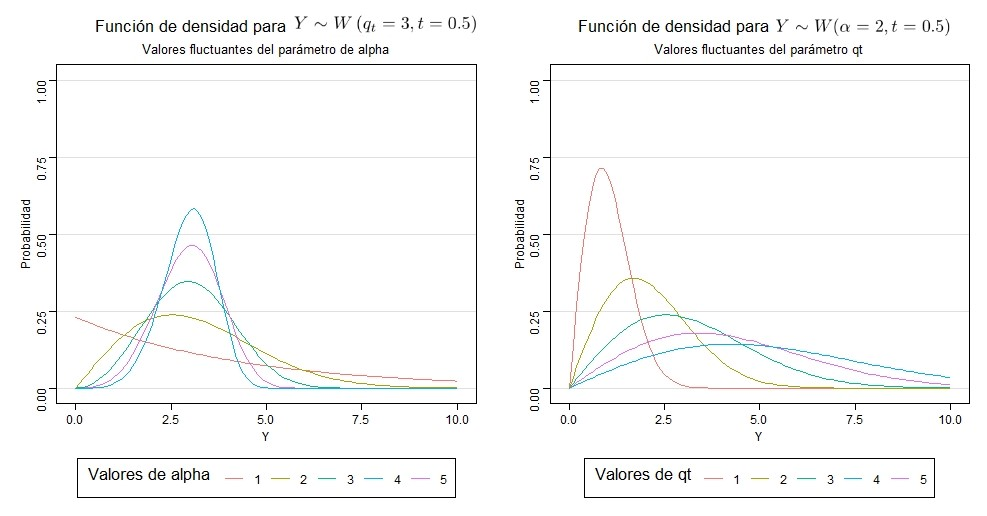
\includegraphics[width=\textwidth]{densidad1}
\caption{Función de densidad de una distribución Weibull bajo la reparametrización propuesta.}
\end{figure}

\noindent Se observa que en la medida que $q_{t}$ aumenta, la distribución incrementa su asimetría hacia la derecha. Ello también sucede, aunque en menor grado, cuando $\alpha$ aumenta. No obstante, se observa que en la medida que $\alpha$ tiende a 0, incrementa la dispersión.

Reexpresando la función acumulada en los términos de la parametrización propuesta, esta tendría la siguiente forma:
\begin{equation} \label{eq:1}
F_{y}\left(y| q_{t},\alpha,t \right)=1-\exp\left( -c(t)\left( \frac{y}{q_{t}} \right)^{\alpha} \right).
\end{equation}
\subsection{Estudio de la parametrización propuesta}

La esperanza y varianza de una variable aleatoria bajo la parametrización Weibull propuesta están dadas bajo la siguiente expresión:
\begin{equation}
E(Y)=\frac{q_{t}}{c(t)^{\frac{1}{\alpha}}}\Gamma\left( 1+\frac{1}{\alpha} \right)
\end{equation}

\begin{equation}
Var(y)=\frac{q_{t}^{2}}{c(t)^{\frac{1}{\alpha}}}\left[ \Gamma\left( 1+\frac{2}{\alpha}\right)-\Gamma\left( 1+\frac{1}{\alpha} \right)^{2} \right]
\end{equation}

Bajo la parametrización propuesta, se observa que para un $\alpha$ fijo el valor esperado se comporta de forma lineal en la medida que aumente el parámetro $q_{t}$ conforme se observa en el cuadro siguiente:

\begin{figure}[H]
	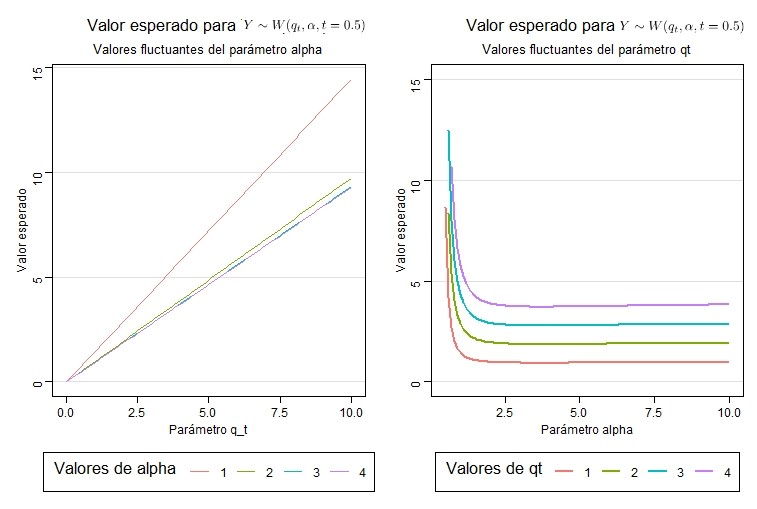
\includegraphics[width=\textwidth]{esperado}
	\caption{Valor esperado de una distribución Weibull bajo la parametrización propuesta.}
\end{figure}
\noindent No obstante, para un $q_{t}$ fijo, lo mismo no se observa en la medida que aumente $\alpha$. Se observa un comportamiento no lineal y asintótico: cuando $\alpha$ tiende a 0, el valor esperado tiende a infinito. Cuando $\alpha$ aumenta, el valor esperado se estabiliza.

En el caso de la varianza se observa que para un $\alpha$ fijo, en la medida que aumente el parámetro $q_{t}$ la varianza aumenta de forma exponencial. No obstante, y como se puede apreciar cuando $q_{t}$ está fijo, en la medida que los valores de $\alpha$ sean pequeños, la varianza incrementa drásticamente. Asimismo, como se aprecia en el cuadro adjunto, la varianza tiende a 0 en la medida que $\alpha$ aumente.

\begin{figure}[H]
	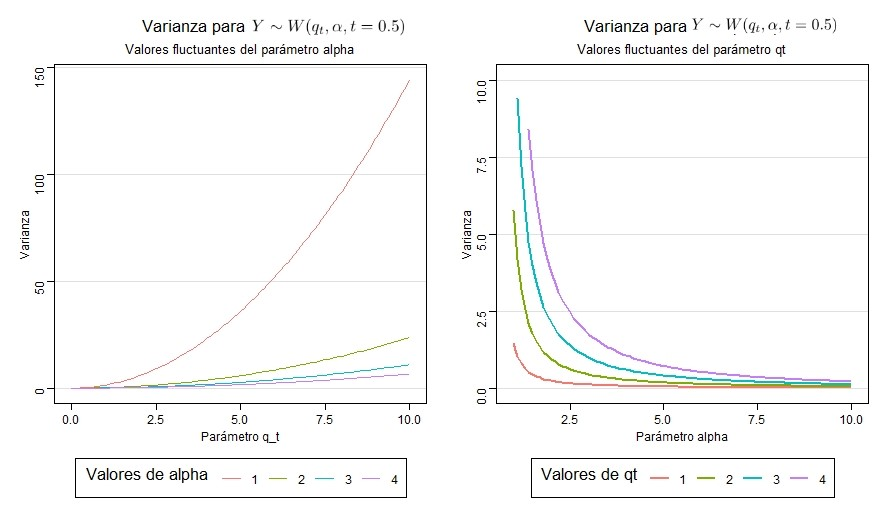
\includegraphics[width=\textwidth]{varianza}
	\caption{Varianza bajo la parametrización propuesta.}
\end{figure}

\chapter{Modelo de regresión cuantílica para datos positivos}
El presente capítulo tiene como objetivo especificar el modelo de regresión cuantílica para datos positivos con censura intervalar. Asimismo, detallamos la estimación de los parámetros desde la perspectiva de inferencia clásica.

\section{Datos positivos con censura intervalar}

Conforme mencionado en la introducción, algunos características de la población pueden solo capturarse en un intervalo por multiplicidad de condiciones. Una de ellas es el derecho a privacidad de las personas, quienes solo desean revelar información sobre si mismas sin exponer mucha información. Caso concreto es el sueldo: una persona no desearía brindar su sueldo específico a alguien desconocido, no obstante puede indicar que su sueldo está en un rango.

Bajo ese contexto, podemos definir una variable aleatoria $z$ como una variable que indica que la variable $y$ se encuentra en el $j$-ésimo intervalo $[L_{j},L_{j+1}]$. Se asume que solamente observamos la variable $z$ mientras que $y$ es una variable latente, que en el ejemplo correspone al sueldo específico de la persona (el cual no ha sido revelado). La variable aleatoria $z$ es una variable cualitativa pues solo se indica el intervalo que la persona responde. Por lo tanto, la podemos definir mediante la siguiente expresión:
\begin{equation}
z = 
	\begin{cases}
		1, L_{1}< y < L_{2} \\
		2, L_{2} \leq y < L_{3} \\
		3, L_{3} \leq y < L_{4} \\
		\vdots \\
		K, L_{K} \leq y < L_{K+1} \\
	\end{cases}
\end{equation}

En dónde $L_1 < L_2 < \cdots < L_{K+1}$, y corresponde a los límites del intervalo, con $L_{1}=0$ y $L_{K+1}=\infty$. La probabilidad de $Z$ está definida bajo la siguiente expresión:
\[P\left( Z=j \right)=P\left(L_{j} \leq y < L_{j+1} \right)\]
\[P\left( Z=j \right)=F\left( L_{j} \right)-F\left( L_{j+1} \right)\]

\noindent dónde $F(\cdot)$ es la función de distribución acumulada de Y. La variable $Z$ que sigue la distribución anteriormente mencionada está denotada por 
$$Z \sim \text{Categórica}(\pi)$$
\noindent dónde $\pi=\left( \pi_{1},\dots,\pi_{k}\right)$y $\pi_{j}=P(Z=j)$.

\section{Modelo de regresión para datos positivos con censura intervalar}

El modelo de regresión cuantílica para datos positivos está dado por lo siguiente:

\[Y_{i} \sim W_{r}\left( q_{t_{i}},\alpha,t \right).\]
\[g\left( q_{t_{i}} \right) = x_{i}^{T}\beta.\]

\noindent en dónde $\beta=\left[ \beta_0,\beta_{1},\dots,\beta_{p} \right]^{T}$ y $x_{i}^{T} =\left[ 1,x_{i1},x_{i2},\dots,x_{ip}, \right]^{T}$. La función $g(\cdot)$ es una función de enlace estrictamente monótona y doblemente diferenciable. En el presente modelo, se utilizará la función de enlace logarítmica. El parámetro de forma $\alpha$, el parámetro $q_{t_{i}}$ y $t$ está definido conforme la sección 2.1. La estimación de los parámetros $\beta$ y $\alpha$ se realizará mediante el método de máxima verosimilitud.

\subsection{Función de verosimilitud}
Consideramos que solo conocemos que $Y_{i}$ se encuentra en un intervalo de $K$ posibles intervalos de la forma $[L_{j},L_{j+1}]$ con $L_1 < L_2 < \dots < L_{K+1}$ y que $Z_{i}=j$ denota que $Y_{i} \in [L_{j},L_{j+1}]$. Por lo tanto, considerando los resultados de la sección 3.1, tenemos que
\[Z_{i} \sim \text{Categórica}(\pi_{i}).\]
\noindent con $\pi_{i}=\left( \pi_{i1},\dots, \pi_{ik} \right)$ tal que
\begin{equation}
\pi_{ij} = F_{y}(L_{j}|q_{t_{i}},\alpha,x) - F_{y}\left( L_{j+1}|q_{t_{i}},\alpha,x \right)
\end{equation}

Entonces la función de verosimilitud de las variables observadas $Z_{1},Z_{2},\dots,Z_{n}$ es dada por lo siguiente:

\[L(\theta)=\prod_{i=1}^{n}\prod_{j=1}^{k} \pi_{ij}^{1\left( Z_{i}=j \right)}.\]

Luego, considerando  [$\psi_{i_{inf}},\psi_{i_{sup}}$] como el intervalo dónde $Y_{i}$ fue observado, podemos escribir la función de verosimilitud como:

\[L\left( \theta\right)=\prod_{i=1}^{n}\left( F(\psi_{i_{sup}}|q_{t_{i}},\alpha,t) - F(\psi_{i_{inf}}|q_{t_{i}},\alpha,t) \right) \]

\[L(\theta)=\sum_{i=1}^{n} \log \left( F(\psi_{i_{sup}}|q_{t_{i}},\alpha,t) - F\left( \psi_{i_{inf}}|q_{t_{i}},\alpha,t \right) \right)\]

\[L(\theta)=\sum_{i}^{n} \log \left( \exp\left( -c(t)\left( \frac{\psi_{i_{inf}}}{e^{x_{i}^{T}\beta}} \right)^{\alpha} - \exp\left( -c(t)\left( \frac{\psi_{i_{sup}}}{e^{x_{i}^{T}\beta}} \right)^{\alpha} \right) \right) \right)\]
\noindent en dónde $c(t)=(-log(1-t))^{\frac{1}{\alpha}}$.

Los estimadores de máxima verosimilitud para los parámetros $\alpha$ y $\beta$ se encuentran maximizando la función anteriormente expuesta. Para ello, obtenemos las gradientes de $\alpha$ y $\beta$, se exponen a continuación (asumiendo que $g(\cdot)$ es la función logaritmo):

\[\frac{\partial L}{\partial \alpha}=\sum_{i=1}^{n} \frac{c(t)}{(\gamma_{i})^{\alpha}(\lambda_{i_{2}}-\lambda_{i_{1}})}\left( (\psi_{i_{sup}})^{\alpha} \log\left( \frac{\psi_{i_{sup}}}{\gamma_{i}} \right) \lambda_{i_{2}} - (\psi_{i_{inf}})^{\alpha} \log\left( \frac{\psi_{i_{sup}}}{\gamma_{i}} \right) \lambda_{i_{1}}\right)\]

\[\frac{\partial L}{\partial \beta_{j}}=\sum_{i=1}^{n} \left(\frac{\alpha c(t) x_{ij}}{(\gamma_{i})^{\alpha}(\lambda_{i_{1}}-\lambda_{i_{2}})}\right) \left( (\psi_{i_{inf}})^{\alpha}\lambda_{i_{1}} - (\psi_{i_{sup}})^{\alpha} \lambda_{i_{2}} \right)\]
\noindent en dónde:
\[ \gamma_{i} = \exp(\eta_{i})\]
\[ \eta_{i} = x_{i}^{T}\beta\]
\[ \lambda_{i_{1}} = \exp\left( -c(t) \left(\frac{\psi_{i_{inf}}}{\gamma_{i}}\right)^{\alpha} \right)\]
\[ \lambda_{i_{2}} = \exp\left( -c(t) \left(\frac{\psi_{i_{sup}}}{\gamma_{i}}\right)^{\alpha} \right)\]

La maximización de dicha la función de log-verosimilitud se realizará mediante métodos de optimización numérica a través del lenguaje de programación R.
	
\chapter{Estudio de Simulación}
El presente capítulo tiene como objetivo ejecutar un estudio de simulación para evaluar si tanto el modelo descrito permite capturar los parámetros de regresión cuantílica bajo censura intervalar. Para evaluar el desempeño de los parámetros obtenidos, evaluaremos el sesgo relativo, error cuadrático medio y la cobertura del intervalo de confianza con un nivel de significancia al 95\%.

Para cada uno de los cuantiles $t=\{0.1, 0.2, 0.3, \dots , 0.9\}$ se realizó la simulación de $n=10000$ valores de las siguientes variables:
\[X_{1} \sim Beta(2,3)\]
\[X_{2} \sim Normal(2,0.5)\]
\[X_{3} \sim Gamma(2,25)\]

En base a estas variables simulamos la variable aleatoria dependiente $Y_{i} \sim W_{r}(q_{t},\alpha,t)$ en donde $q_{t}$ está definida de la siguiente forma:
\[q_{t} = e^{X^{T}\beta}, X = \{1,X_{1},X_{2},X_{3}\}\]

Para propósitos de la simulación, se fijaron los parámetros siguientes:
\[\alpha=2\]
\[\beta_{0}=0.5\]
\[\beta_{1}=0.3\]
\[\beta_{2}=0.6\]
\[\beta_{3}=0.8\]

Una vez generada la variable aleatoria $ Y_{i} $, se censuró esta información en base al criterio de particiones iguales hasta determinado el percentil 80. Esto se debe a que la variable respuesta $ Y_{i} $ tiene colas pesadas. Ver seudocódigo en la siguiente:

Seudocódigo aquí

Se tomó en cuenta las siguientes consideraciones:

\begin{itemize}
    \item Puntos iniciales
    \item Cálculo de 
\end{itemize}}

Finalmente, se observa que:

Ver cuadro a continuación

\chapter{Aplicaciones}

Este capítulo se completará en posteriores entregas.

\chapter{Conclusiones}

Este capítulo se entregará en posteriores entregas.
\chapter{Bibliografía}


Weibull, Waloddi. "A statistical distribution function of wide applicability"\textit{ASME Journal of Applied Mechanics.}.1951, pp. 293-297.

\

Fahrmeir, Ludwig. Kneib, Thomas. Lang, Stefan. Marx, Brian. \textit{Regression: Models, Methods and Applications.} 2013. Springer.

\

Du, Xiuli. Feng, Yanqin. Zhou, Xiuqing. "Quantile regression for interval censored data". \textit{Communications in Statistics - Theory and Methods.} 2015, pp. 3848-3863.

\

Koenker, Roger. Basset, Gilbert Jr. Regression Quantiles. 1978.

\

Sal y Rosas, Víctor. Moscoso-Porras, Miguel. Ormeño, Rubén. Artica, Fernando. Bayes, Cristian Luis. Miranda, Jaime. Gender Income Gap among physicians and nurses in Perú: a nationwide assessment. \textit{The Lancet.} 2019.
\end{document}
